\begin{figure*}[t]
\centering
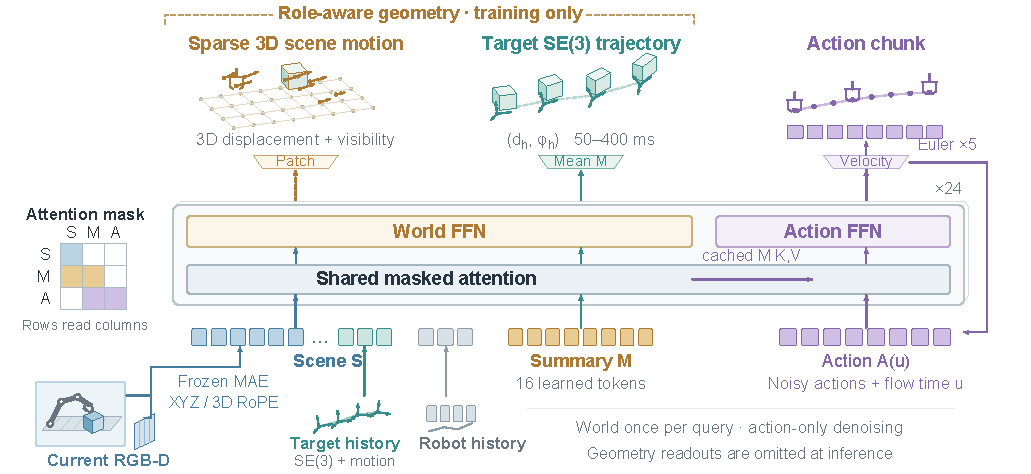
\includegraphics[width=\textwidth]{figures/Fig2/fig2_se3wam.pdf}
\caption{\textbf{\ours architecture.} Read from bottom to top.
RGB-D and target/robot histories form $S=212$ scene tokens. One backbone shares
masked attention; actions read summary tokens $M$. Training-only linear heads
supervise sparse whole-scene 3D flow/visibility from patches and target SE(3)
from the mean summary. Geometry is GT from one recorded \bench{} conveyor
episode: a workspace crop of the $14\times14$ grid at 400\,ms and eight orange
pose axes at 50--400\,ms. Blue axes show history; the purple path illustrates
actions with recorded expert EEF states. RGB scenes are Blender renders;
none of these illustrations is a model prediction. At inference, the entire
dashed region is skipped and world keys/values are cached across \cfgEuler{} action Euler steps.}
\label{fig:architecture}
\end{figure*}
